\documentclass[12pt]{article}
\usepackage[margin=1in]{geometry}
\usepackage{setspace}
\usepackage[T1]{fontenc}
\usepackage{newtxtext,newtxmath}
\usepackage{graphicx}
\usepackage{float}
\usepackage{booktabs}
\usepackage{tabularx}
\usepackage{array}
\usepackage{ragged2e}
\usepackage{caption}
\usepackage[table]{xcolor}
\usepackage{hyperref}

\doublespacing
\setlength{\parindent}{0pt}
\setlength{\parskip}{0.5em}
\setlength{\tabcolsep}{4.5pt}
\renewcommand{\arraystretch}{1.16}
\setlength{\emergencystretch}{2em}
\captionsetup{font={small,stretch=1},labelfont=bf}

\definecolor{stagecollect}{HTML}{365C8D}
\definecolor{stageclean}{HTML}{2E7D6E}
\definecolor{stageprep}{HTML}{C97A2B}
\definecolor{stagemine}{HTML}{7B4FA0}
\definecolor{lightcollect}{HTML}{EAF1F8}
\definecolor{lightclean}{HTML}{E8F4F1}
\definecolor{lightprep}{HTML}{FBF1E4}
\definecolor{lightmine}{HTML}{F1E9F8}
\definecolor{tableheader}{HTML}{F2F2F2}

\newcolumntype{L}[1]{>{\RaggedRight\arraybackslash}p{#1}}
\newcolumntype{Y}{>{\RaggedRight\arraybackslash}X}

\newcommand{\stagecell}[2]{\cellcolor{#1!14}\textcolor{#1}{\textbf{#2}}}
\newcommand{\metriccell}[2]{\cellcolor{#1!14}\textbf{#2}}
\DeclareRobustCommand{\artifact}[1]{\texttt{#1}}

\title{Materials and Methods Draft\\Mouse DRG RNA-seq Follow-up Project}
\author{Piter Garcia}
\date{Draft prepared for BIOL550}

\begin{document}
\maketitle

\section{Materials and Methods}

This project reanalyzed mouse DRG bulk RNA-seq after sciatic nerve injury using four stages: \textbf{Data Collection}, \textbf{Data Cleaning}, \textbf{Data Preparation}, and \textbf{Data Analysis and Interpretation}. The working subset comprised 20 NovaSeq X paired-end libraries from \artifact{SRP618841} (BioProject \artifact{PRJNA1322439}; GEO \artifact{GSE243308}) organized into a balanced side-by-genotype design before QC, alignment, and DE modeling began.

\begin{figure}[H]
\centering
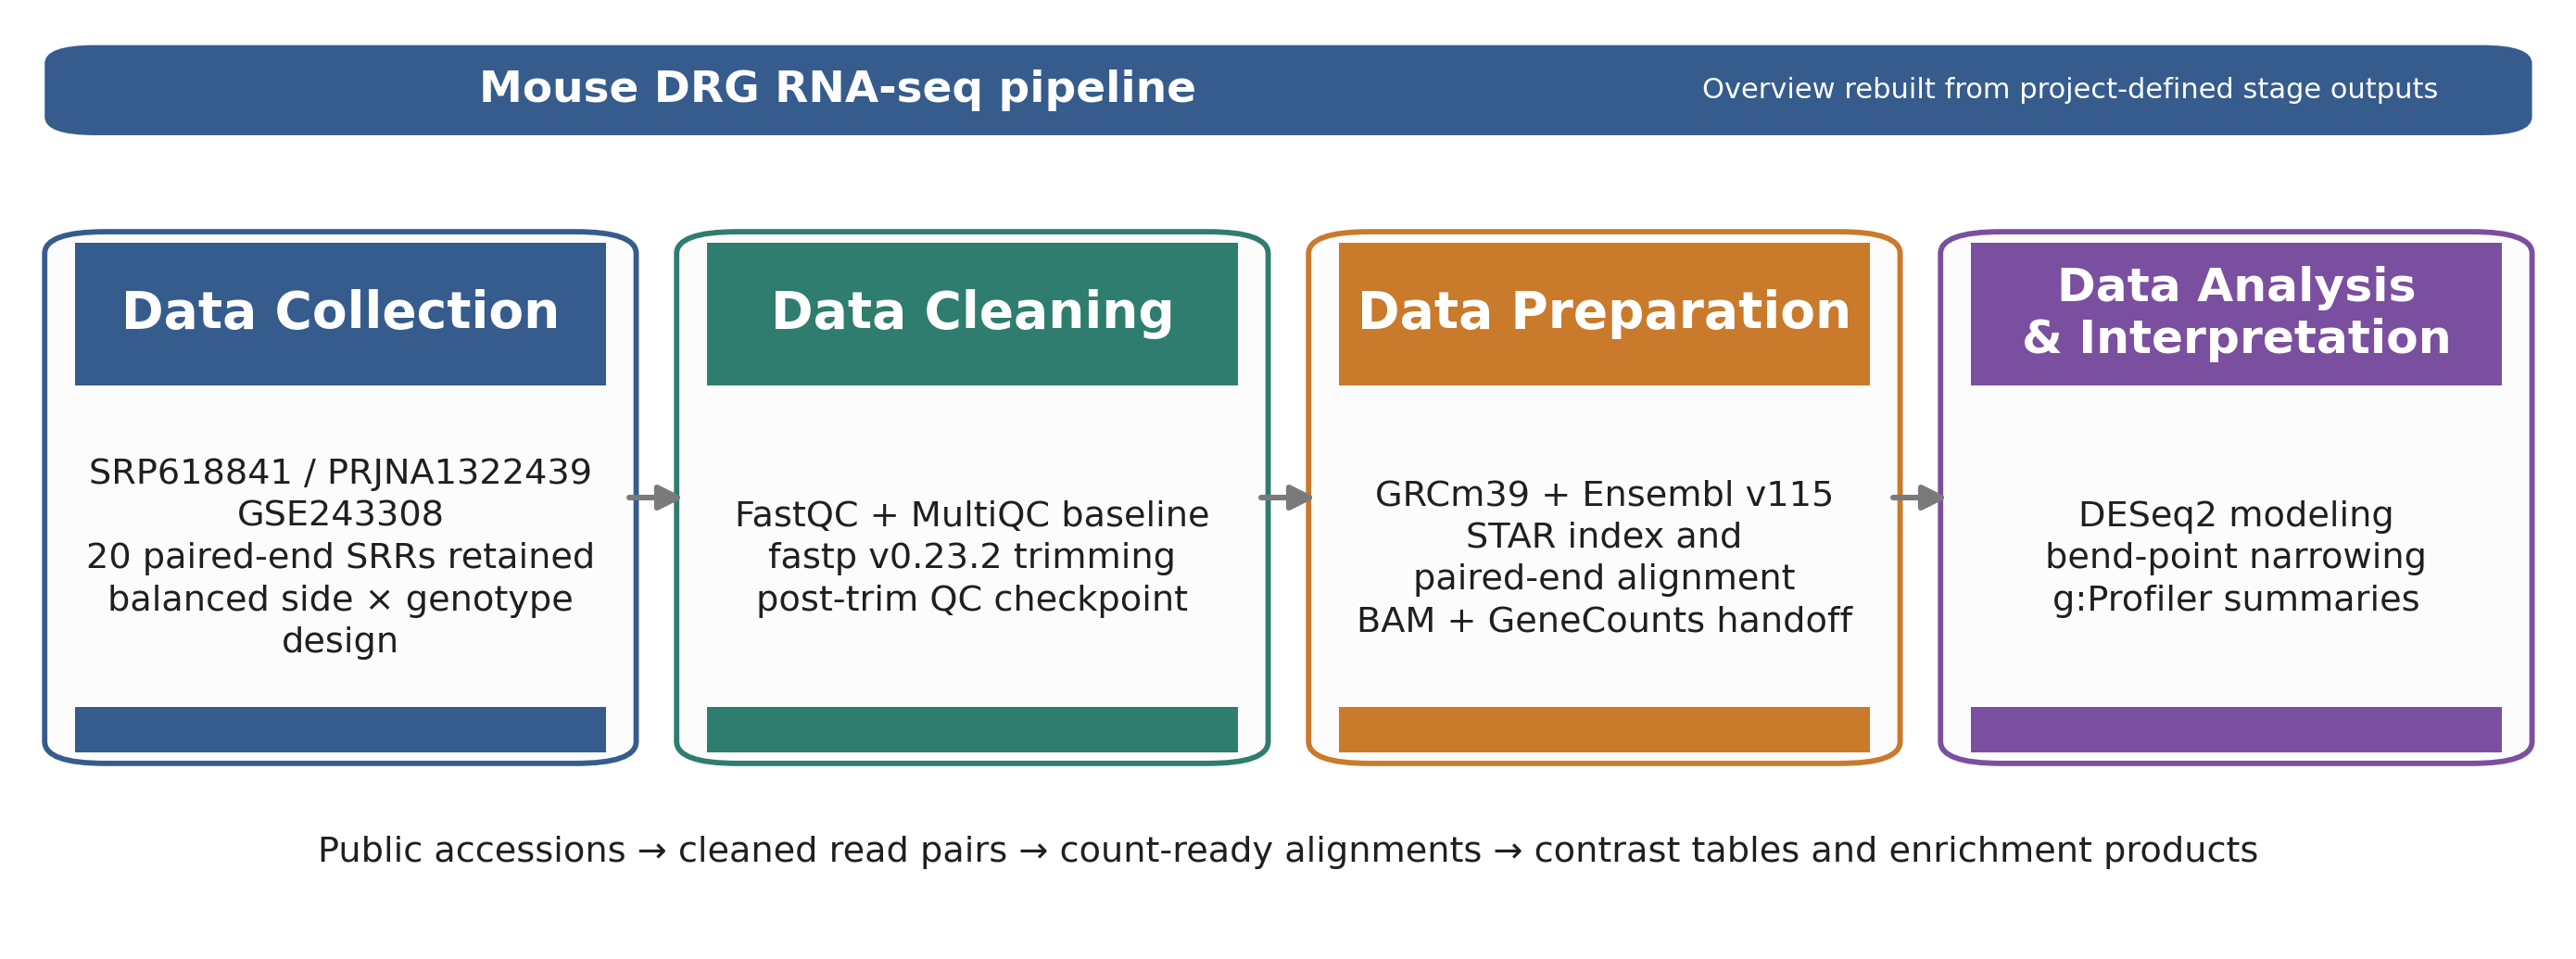
\includegraphics[width=1.02\textwidth]{assets_methods/overview_pipeline_stage.png}
\caption{Overview ribbon summarizing the four computational stages and their stage-owned handoffs in the \artifact{mouse\_new} workflow.}
\label{fig:overall_pipeline}
\end{figure}

\begin{table}[H]
\centering
\begin{singlespace}
\fontsize{7.0}{7.7}\selectfont
\caption{Pipeline checkpoint table used to anchor the Methods section to stage-specific evidence.}
\label{tab:pipeline_checkpoint}
\begin{tabularx}{\textwidth}{Y Y Y Y Y}
\toprule
\rowcolor{tableheader}
\textbf{Stage} & \textbf{Primary artifacts} & \textbf{Core tools} & \textbf{Checkpoint metric} & \textbf{Handoff} \\
\midrule
\stagecell{stagecollect}{Collection} &
sample table; family sheet &
\artifact{prefetch} + \artifact{fasterq-dump} &
\metriccell{stagecollect}{20 SRRs retained; 4 balanced subgroups ($n=5$ each)} &
\artifact{FASTQ.gz} pairs + manifest \\

\stagecell{stageclean}{Cleaning} &
QC heatmap; severity delta &
\artifact{FastQC} + \artifact{MultiQC} + \artifact{fastp} &
\metriccell{stageclean}{raw adapter-content failures resolved after trimming} &
trimmed read pairs plus per-sample QC reports \\

\stagecell{stageprep}{Preparation} &
unique-mapping plot; STAR median summary &
\artifact{STAR} + \artifact{GeneCounts} &
\metriccell{stageprep}{93.24\% median unique mapping; 3.82\% median \artifact{noFeature}} &
sorted BAMs, STAR logs, count tables, and family matrix \\

\stagecell{stagemine}{Analysis} &
filtering summary\\
analysis summary\\
g:Profiler source tables &
\artifact{DESeq2} + bend-point + \artifact{g:Profiler} &
\metriccell{stagemine}{78{,}334 $\rightarrow$ 21{,}481 genes after filtering; 5 modeled contrasts} &
DE tables, bend-point follow-up sets, and enrichment summaries \\
\bottomrule
\end{tabularx}
\end{singlespace}
\end{table}

\subsection{Data Collection: SRA Acquisition and Sample Organization}
The project started from the published DRG RNA-seq study \artifact{SRP618841}, which is linked to BioProject \artifact{PRJNA1322439} and GEO series \artifact{GSE243308}. Public runs were retrieved through the project's acquisition wrappers around \artifact{prefetch} and \artifact{fasterq-dump}, and the local workflow retained 20 paired-end NovaSeq X libraries from the 1-day-post-injury DRG subset. The accession lineage matters here because the downstream paper draft needs a precise record of what was reanalyzed, not just a verbal reference to ``the mouse dataset.''

Once the runs were local, metadata were consolidated into a design-aware sample table rather than being left as file-name strings. Each retained sample was tagged with \artifact{side\_class} (\artifact{ipsi} or \artifact{contra}), \artifact{geno\_class} (\artifact{ff} or \artifact{cre}), and the derived \artifact{condition\_family}. That step established the balanced 2$\times$2 design that later drove both the DESeq2 model and the interpretation strategy emphasized in class discussions.

\begin{figure}[H]
\centering
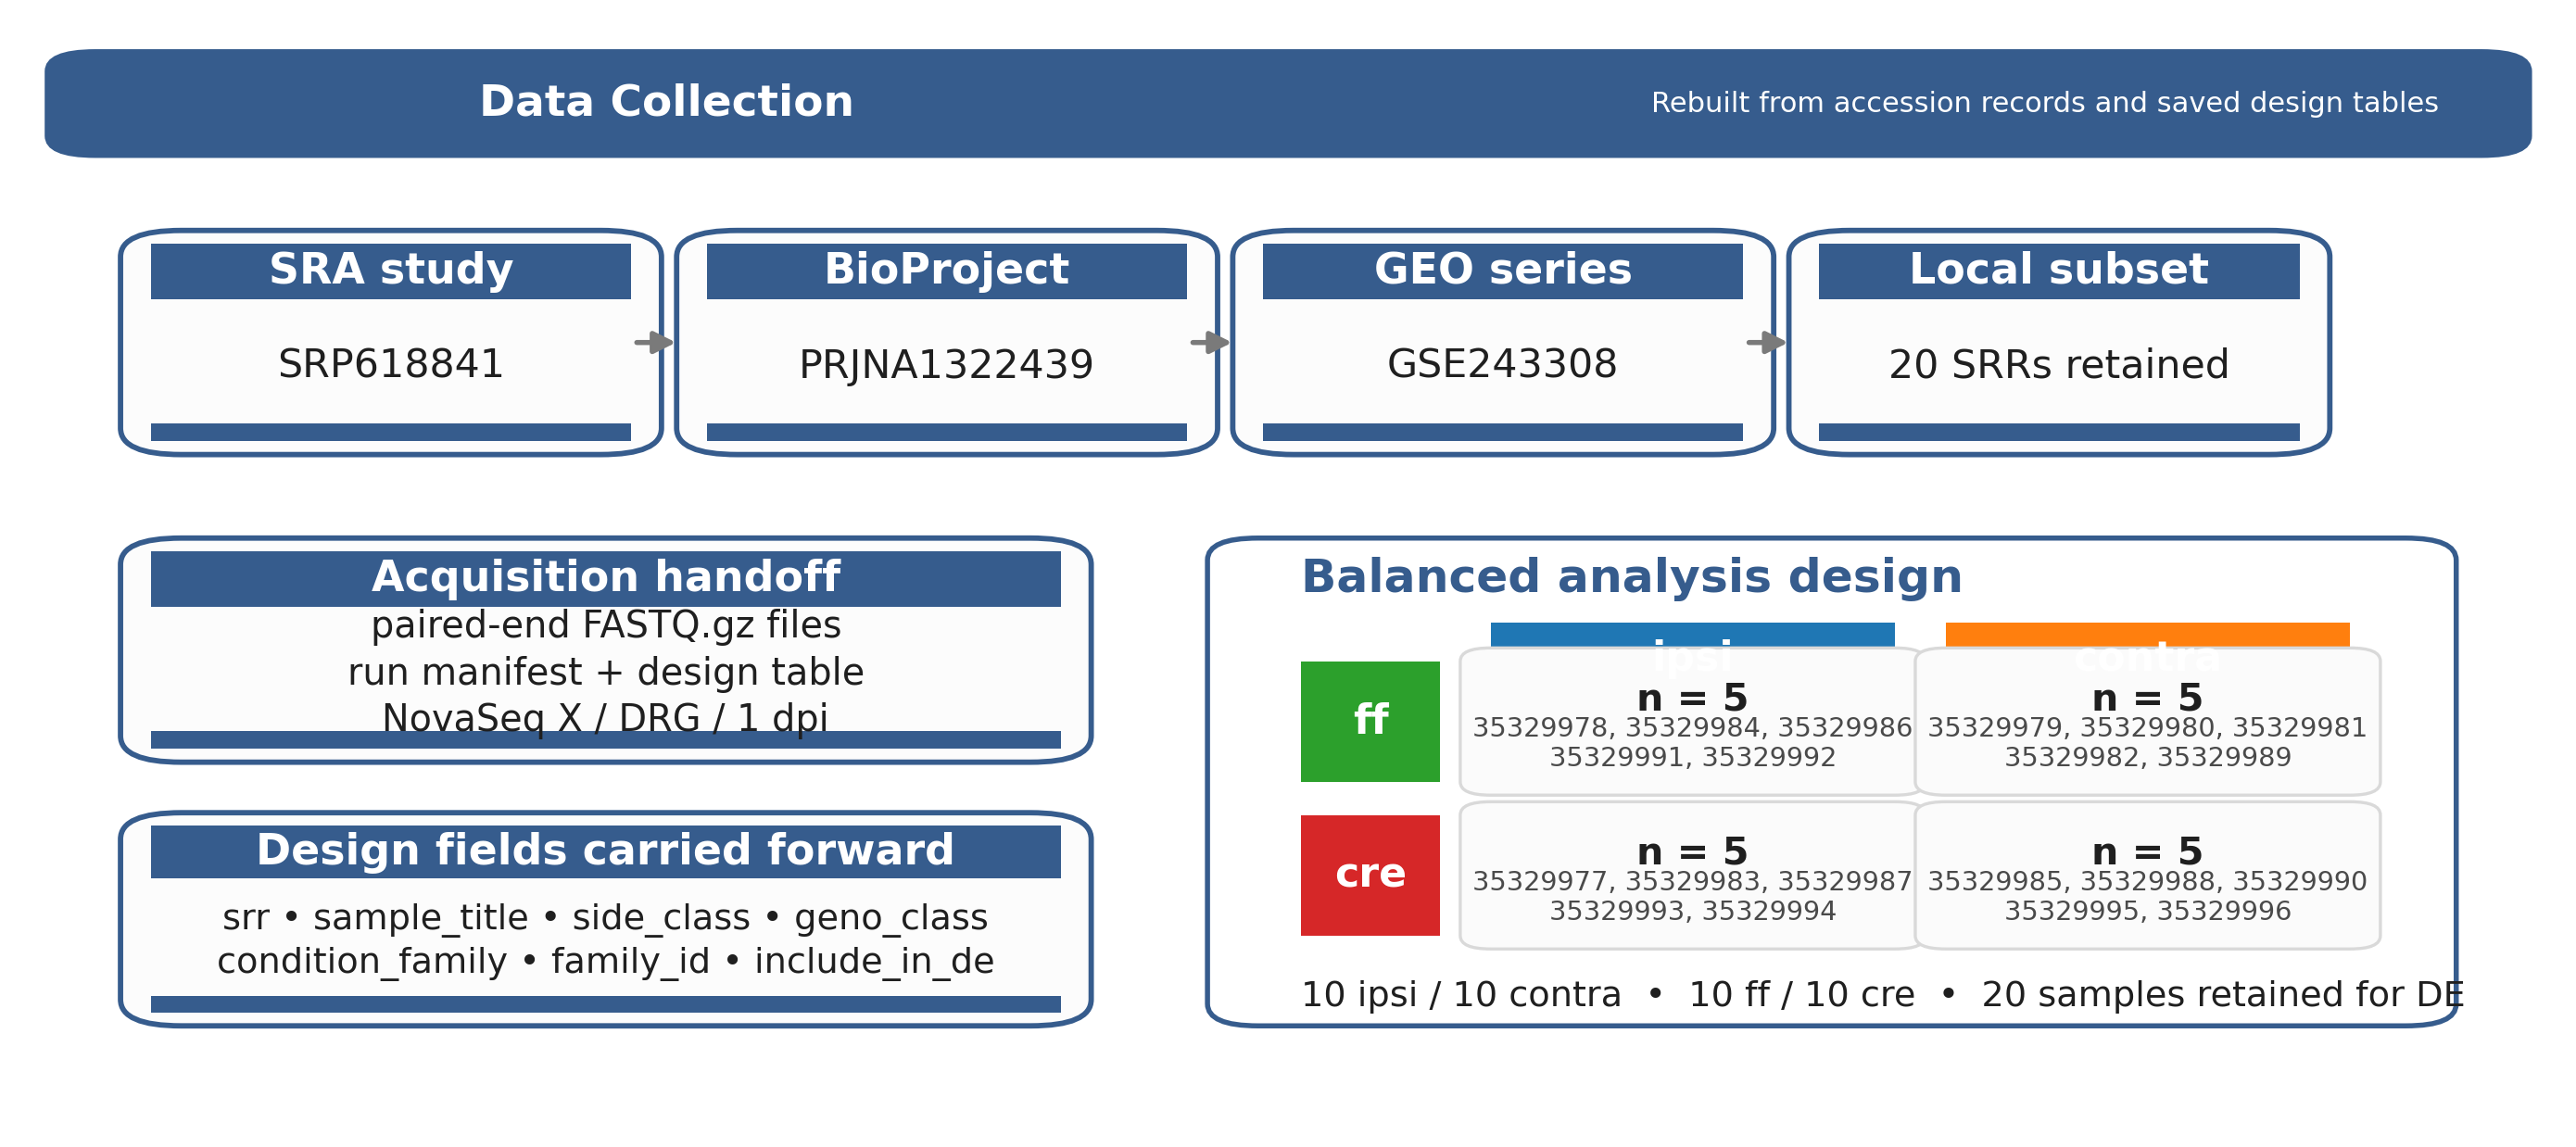
\includegraphics[width=1.02\textwidth]{assets_methods/data_collection_stage.png}
\caption{Rebuilt Data Collection stage figure derived from the saved project metadata and design tables.}
\label{fig:data_collection}
\end{figure}

\begin{table}[H]
\centering
\begin{singlespace}
\fontsize{7.2}{8.1}\selectfont
\caption{Data Collection stage table.}
\label{tab:data_collection}
\begin{tabularx}{\textwidth}{Y Y Y Y Y}
\toprule
\rowcolor{tableheader}
\textbf{Substage} & \textbf{Input} & \textbf{Tool} & \textbf{Checkpoint artifact / evidence} & \textbf{Why it mattered} \\
\midrule
\stagecell{stagecollect}{Study provenance} &
public accession records &
SRA / GEO review &
accession lineage shown in Figure~\ref{fig:data_collection}: \artifact{SRP618841} $\rightarrow$ \artifact{PRJNA1322439} $\rightarrow$ \artifact{GSE243308} &
anchors the Methods section to the exact source study \\

\stagecell{stagecollect}{Run acquisition} &
public SRA runs &
\artifact{prefetch}\\
\artifact{fasterq-dump} &
paired-end \artifact{FASTQ.gz} files plus the local run manifest; 20 retained SRRs from the DRG / NovaSeq X subset &
creates the fixed read set used throughout the pipeline \\

\stagecell{stagecollect}{Design mapping} &
run manifest + sample titles &
local manifest assembly &
design table and family sample sheet; 5 samples in each subgroup &
makes the side/genotype structure explicit before PCA and DE modeling \\
\bottomrule
\end{tabularx}
\end{singlespace}
\end{table}

\subsection{Data Cleaning: Quality Control and Read Trimming}
Raw read quality was reviewed with \artifact{FastQC}, and the cohort-level summaries were consolidated with \artifact{MultiQC}. This stage was not treated as a one-line preprocessing checkbox; instead, the project preserved before/after QC artifacts so that any improvement introduced by trimming could be demonstrated and not merely asserted. The local workflow retained \artifact{fastp} v0.23.2 as the canonical cleanup tool because it handled paired-end adapter detection, tail trimming, and general read cleanup more cleanly than the legacy baseline while keeping the pipeline reproducible.

The retained \artifact{fastp} configuration used paired-end adapter detection, poly-G cleanup, a mean-quality cutoff of 20, a minimum retained length of 30 bases, and per-sample HTML/JSON reporting. In the stage figure, the left panel is the saved module-status heatmap and the right panel is the saved SRR-level severity-change plot; together they show that the trimming stage changed the QC state of the libraries in a consistent cohort-level direction before alignment began.

\begin{figure}[H]
\centering
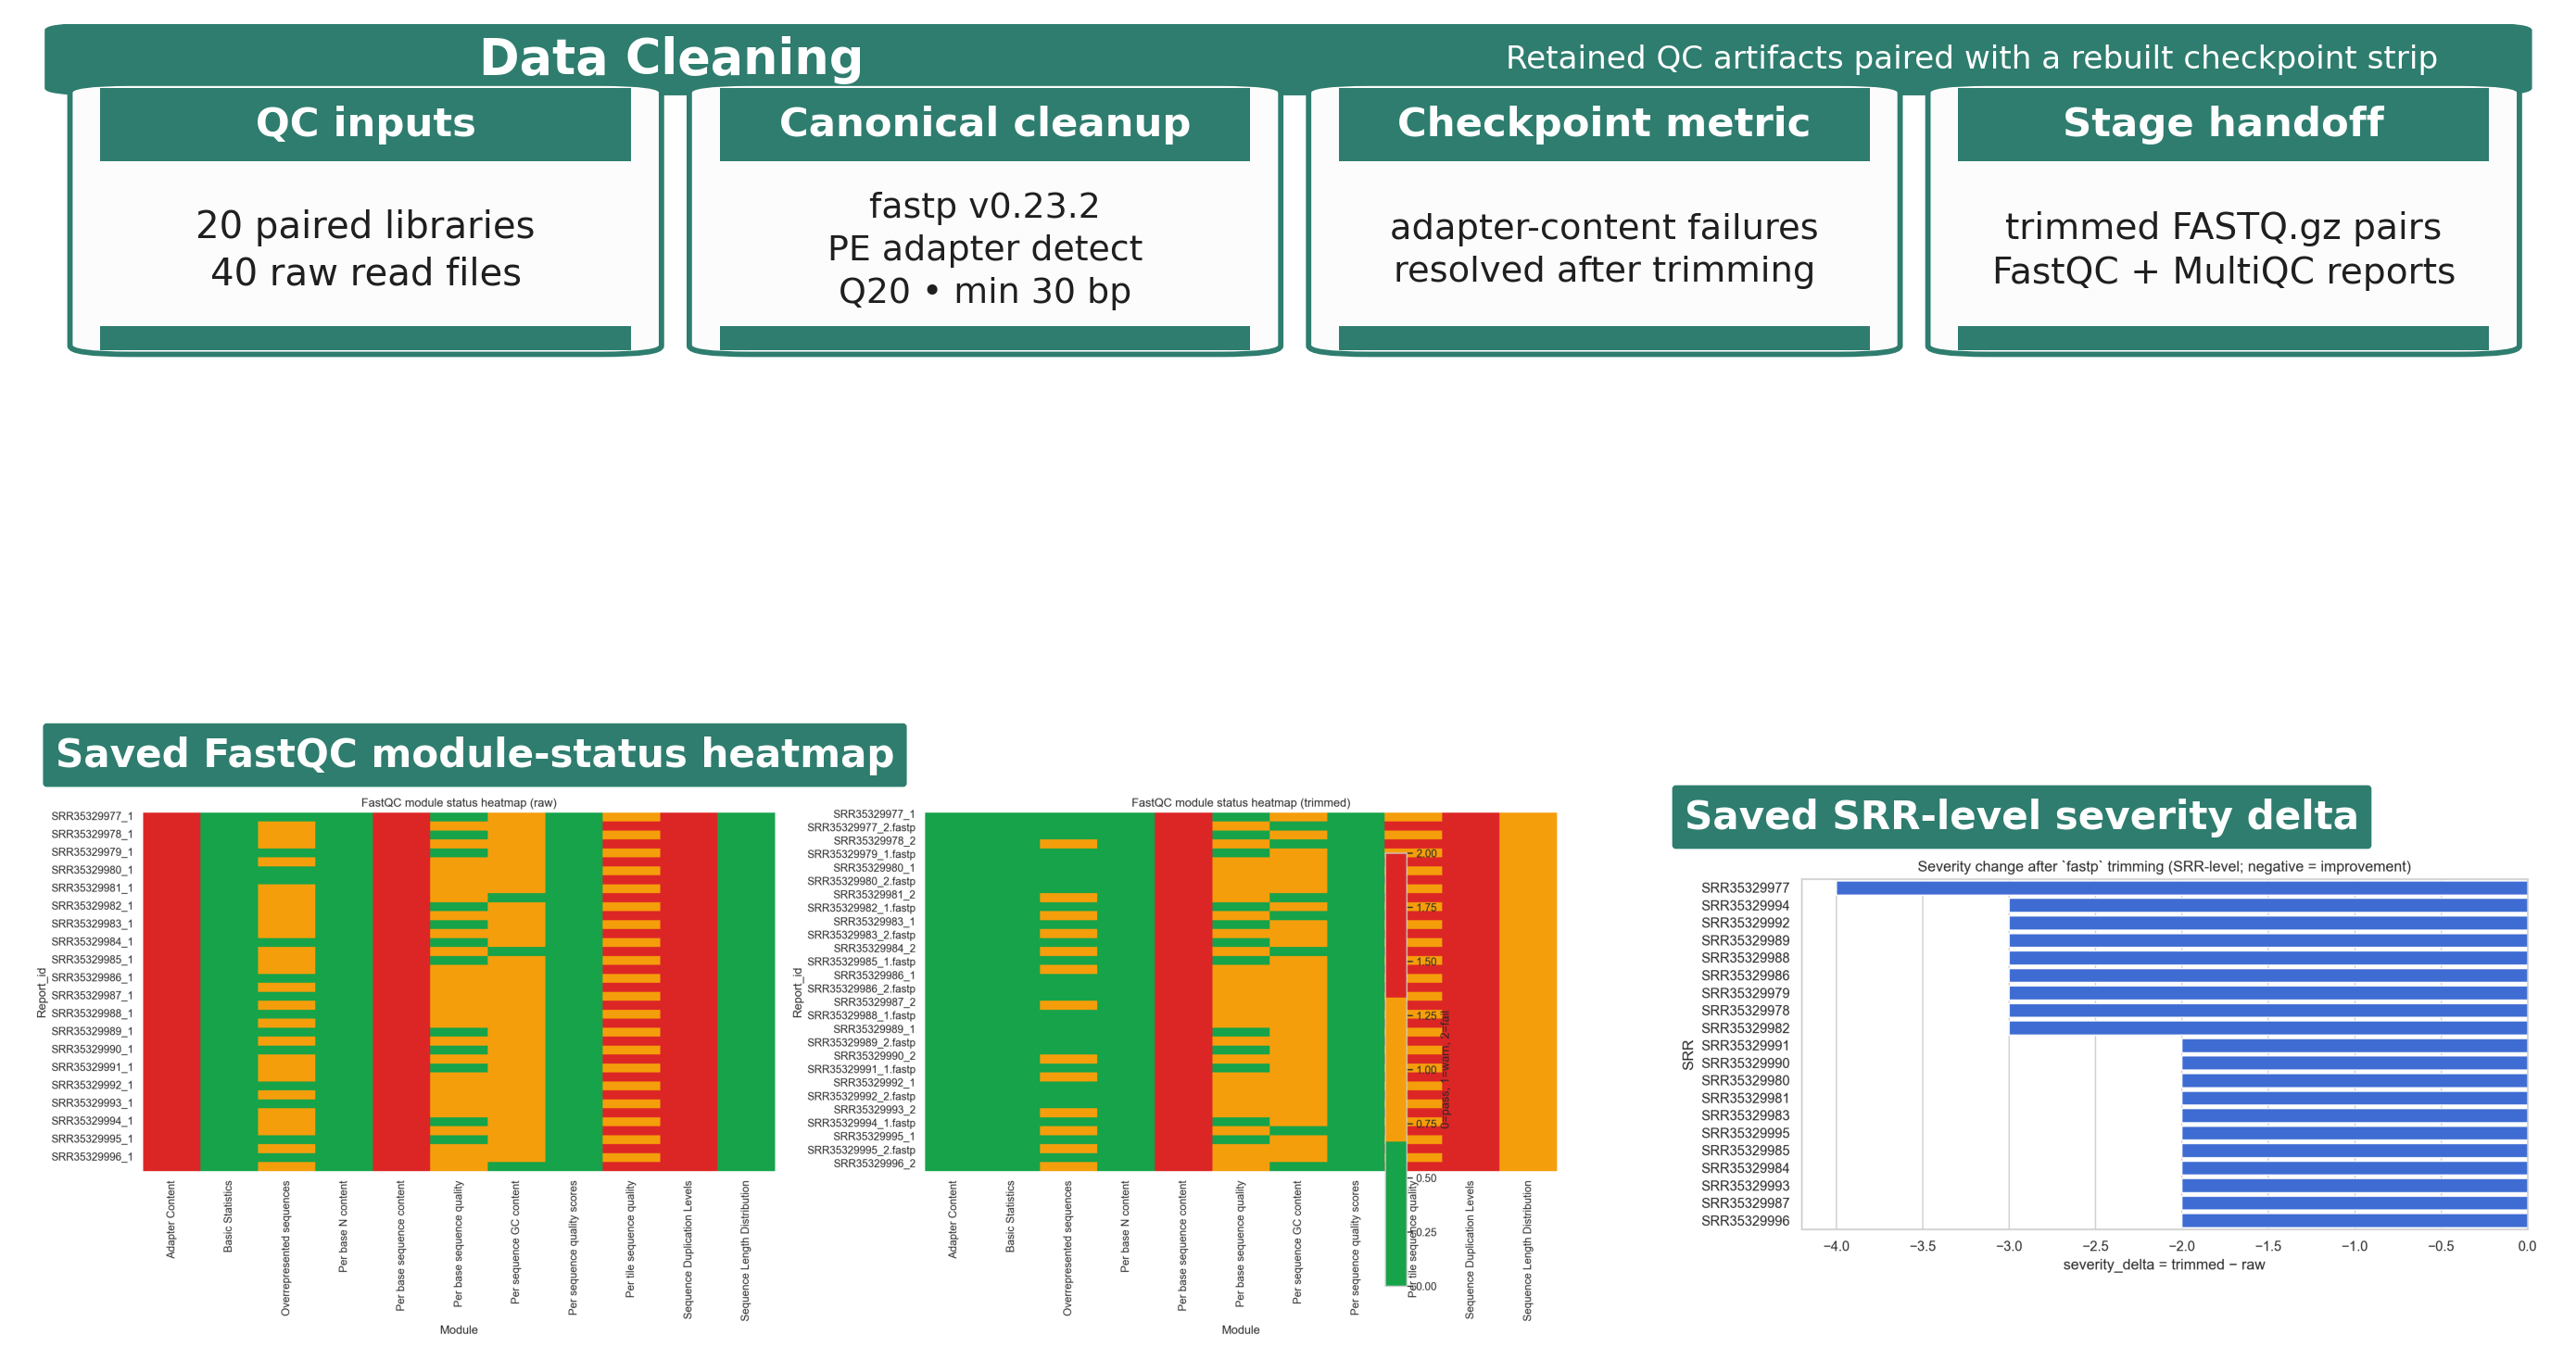
\includegraphics[width=1.04\textwidth]{assets_methods/data_cleaning_stage.png}
\caption{Data Cleaning stage figure using retained QC artifacts and a rebuilt checkpoint strip.}
\label{fig:data_cleaning}
\end{figure}

\begin{table}[H]
\centering
\begin{singlespace}
\fontsize{7.2}{8.1}\selectfont
\caption{Data Cleaning stage table.}
\label{tab:data_cleaning}
\begin{tabularx}{\textwidth}{Y Y Y Y Y}
\toprule
\rowcolor{tableheader}
\textbf{Substage} & \textbf{Input} & \textbf{Tool} & \textbf{Checkpoint artifact / evidence} & \textbf{Why it mattered} \\
\midrule
\stagecell{stageclean}{Raw QC} &
raw paired-end reads &
\artifact{FastQC} + \artifact{MultiQC} &
raw module-status heatmap and cohort QC summary; adapter-content failures across all 40 raw read files &
establishes the baseline quality state before trimming \\

\stagecell{stageclean}{Read trimming} &
raw \artifact{FASTQ.gz} pairs &
\artifact{fastp} v0.23.2 &
trimmed read pairs\\
per-sample HTML/JSON reports; PE adapter detect, Q20 cutoff, min length 30 bp, poly-G trimming &
standardizes cleanup across all retained libraries \\

\stagecell{stageclean}{Post-trim checkpoint} &
trimmed read pairs &
\artifact{FastQC} + \artifact{MultiQC} &
saved SRR-level severity summary; all retained severity deltas shifted negative after trimming &
justifies using the cleaned reads, not the raw reads, for alignment \\
\bottomrule
\end{tabularx}
\end{singlespace}
\end{table}

\subsection{Data Preparation: Reference Selection and Alignment}
The cleaned read pairs were aligned against the \textit{Mus musculus} \artifact{GRCm39} primary assembly with the matching Ensembl release 115 annotation. The reference pair used in the local workflow was \artifact{Mus\_musculus.GRCm39.dna.primary\_assembly.fa} plus \artifact{Mus\_musculus.GRCm39.115.gtf}, and a STAR genome index was built with \artifact{sjdbOverhang = 150} to match the 151-bp paired-end reads. STAR was run with gzip-aware input handling, coordinate-sorted BAM output, and \artifact{GeneCounts} enabled so that the same alignment pass also generated per-sample count tables.

This stage functions as the bridge between cleaned reads and inferential modeling. Each sample produced three checkpoint artifacts that mattered downstream: a sorted BAM, a STAR \artifact{Log.final.out} summary, and a \artifact{ReadsPerGene.out.tab} file. The figure below keeps one retained alignment plot---unique mapping by sample---and pairs it with rebuilt metric cards from the STAR summary tables so the stage is represented by actual alignment evidence rather than by a generic alignment cartoon.

\begin{figure}[H]
\centering
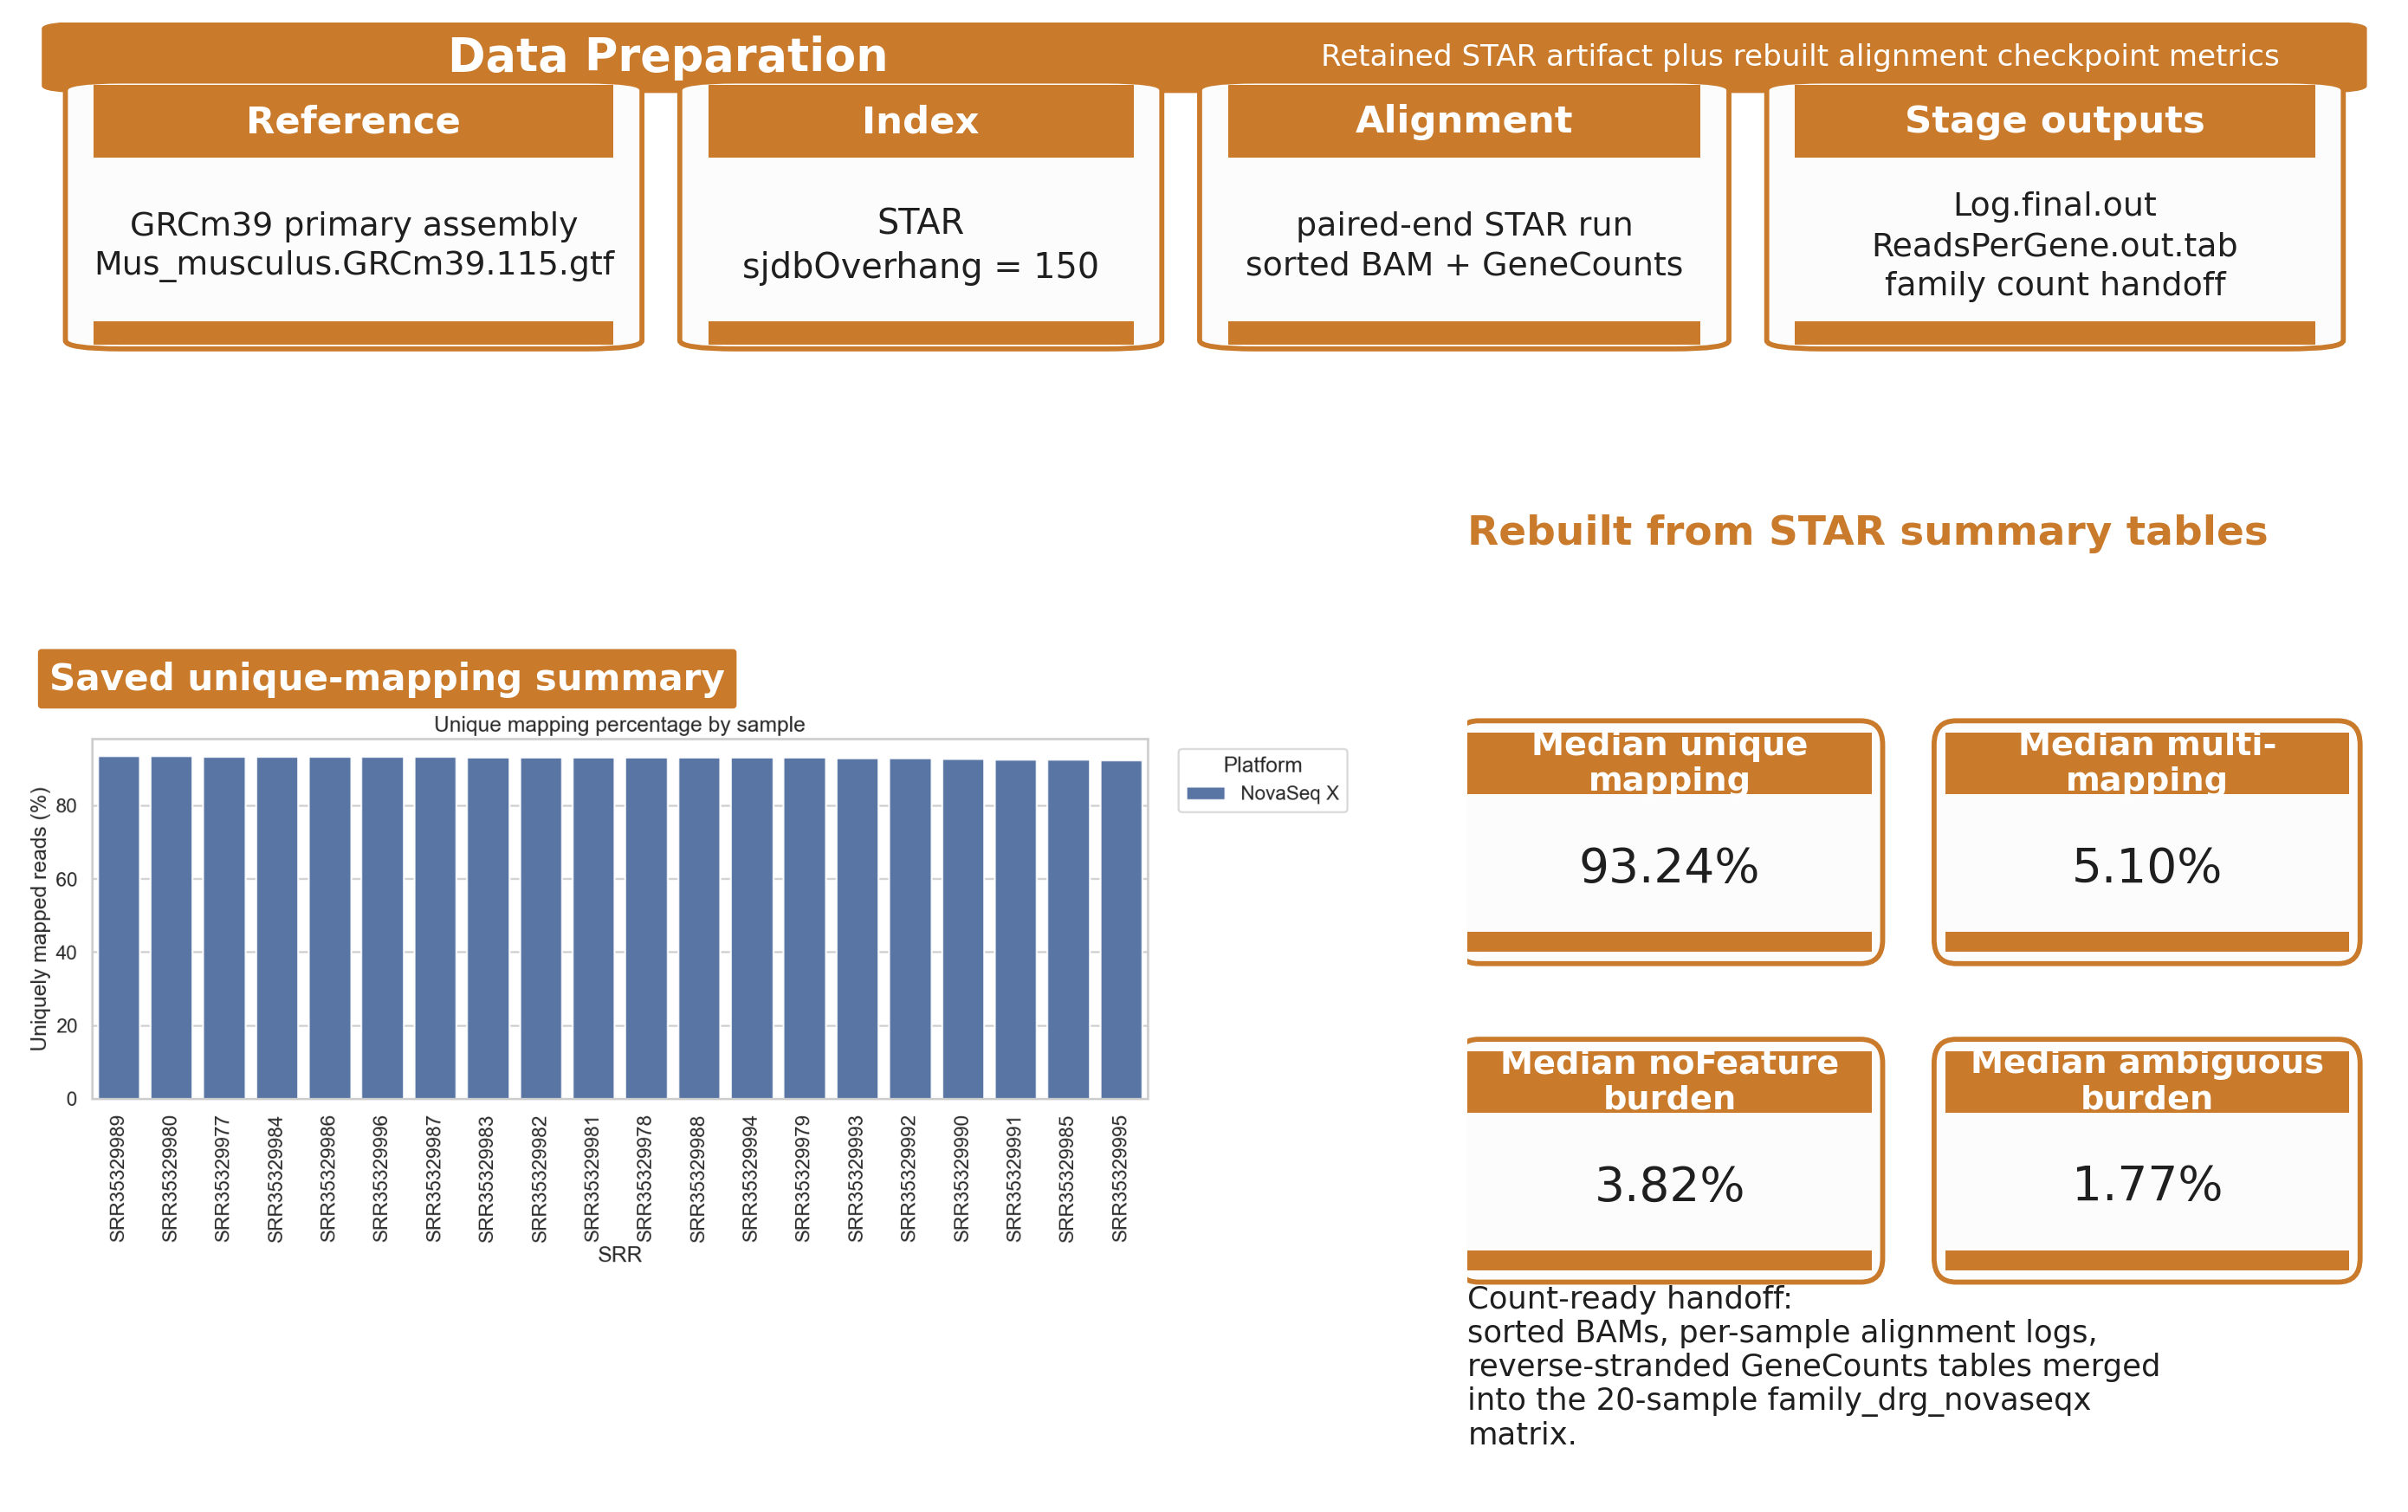
\includegraphics[width=1.04\textwidth]{assets_methods/data_preparation_stage.png}
\caption{Data Preparation stage figure built from retained STAR outputs and rebuilt alignment checkpoint metrics.}
\label{fig:data_preparation}
\end{figure}

\begin{table}[H]
\centering
\begin{singlespace}
\fontsize{7.2}{8.1}\selectfont
\caption{Data Preparation stage table.}
\label{tab:data_preparation}
\begin{tabularx}{\textwidth}{Y Y Y Y Y}
\toprule
\rowcolor{tableheader}
\textbf{Substage} & \textbf{Input} & \textbf{Tool} & \textbf{Checkpoint artifact / evidence} & \textbf{Why it mattered} \\
\midrule
\stagecell{stageprep}{Reference choice} &
mouse genome + annotation &
Ensembl reference selection &
reference FASTA/GTF pair for \artifact{GRCm39} primary assembly + Ensembl v115 annotation &
locks the coordinate system used by STAR and downstream counts \\

\stagecell{stageprep}{STAR index \& run} &
trimmed read pairs + reference &
\artifact{STAR} &
sorted BAM, \artifact{Log.final.out}, and \artifact{ReadsPerGene.out.tab}; \artifact{sjdbOverhang = 150} and paired-end alignment/counting in one run &
produces the alignment checkpoint and the count-ready artifacts in one run \\

\stagecell{stageprep}{Alignment checkpoint} &
saved STAR summaries &
local alignment review &
retained unique-mapping plot plus the STAR median summary table; unique 93.24\%, multi 5.10\%, \artifact{noFeature} 3.82\%, ambiguous 1.77\% &
confirms the cleaned reads mapped well enough to move into DESeq2 \\

\stagecell{stageprep}{Count handoff} &
per-sample count outputs &
local merge scripts / notebooks &
family-level count matrix for \artifact{family\_drg\_novaseqx}; 20 samples retained in the final family matrix &
converts per-sample STAR outputs into the DE-ready family matrix \\
\bottomrule
\end{tabularx}
\end{singlespace}
\end{table}

\subsection{Data Analysis and Interpretation: Differential Expression and Functional Analysis}
The merged family count matrix was modeled with \artifact{DESeq2} using the explicit side/genotype design carried forward from the sample manifest. Prior to modeling, low-support genes were filtered, reducing the tested set from 78{,}334 genes to 21{,}481 while retaining all 20 DRG samples. The workflow then evaluated five contrasts: \artifact{ipsi\_vs\_contra\_in\_ff}, \artifact{ipsi\_vs\_contra\_in\_cre}, \artifact{geno\_in\_contra}, \artifact{geno\_in\_ipsi}, and \artifact{interaction}. PCA, MA plots, volcano plots, and heatmaps were generated at this stage, but they are reserved for the Results section.

To keep very large DE lists from becoming unstructured gene dumps, the workflow added a bend-point rule on the ordered adjusted-\textit{p}-value curve for each contrast. The resulting follow-up sets are therefore reported alongside the \artifact{padj < 0.05} counts rather than treated as guaranteed subsets of them. In practice, this retained 709 and 870 genes for the two primary side-specific contrasts. Those bend-point-selected sets were then submitted to \artifact{g:Profiler} using GO Biological Process, KEGG, and Reactome layers. The stage figure below summarizes the filtered modeling inputs, contrast-level output counts, and enrichment-source layers without reusing the Results figures.

\begin{figure}[H]
\centering
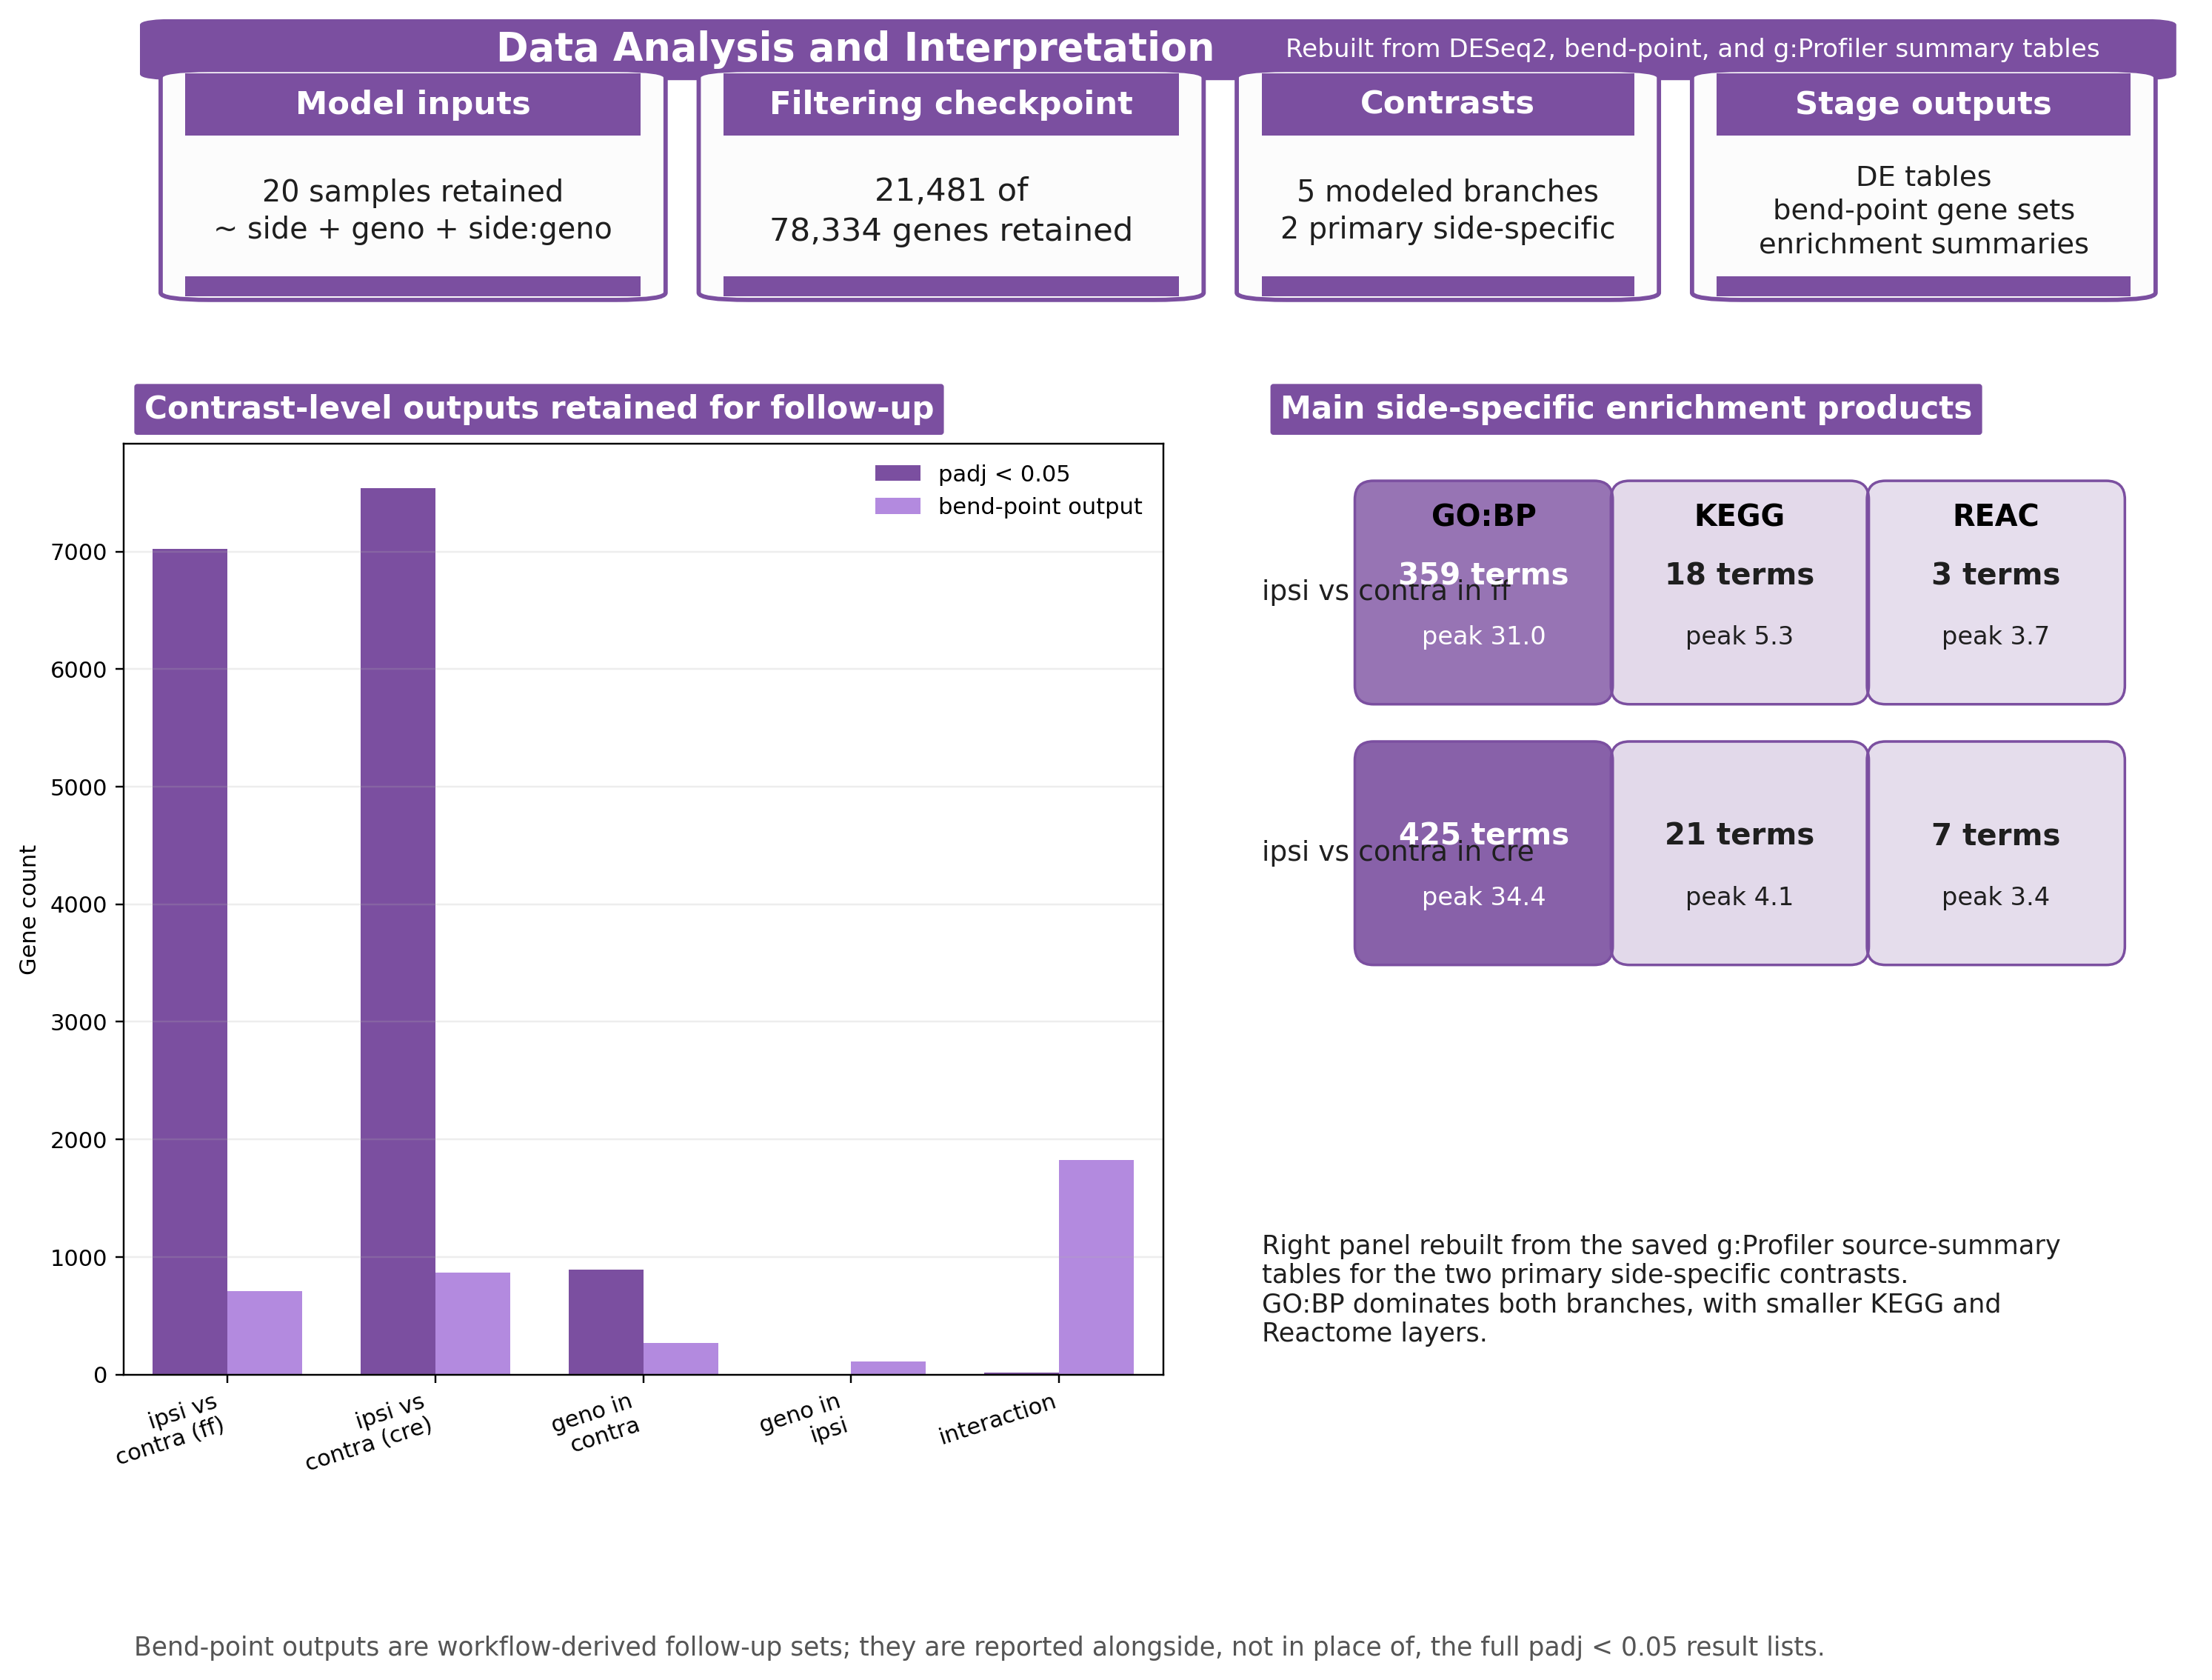
\includegraphics[width=1.04\textwidth]{assets_methods/data_mining_stage.png}
\caption{Rebuilt Data Analysis and Interpretation stage figure derived from saved \artifact{DESeq2}, bend-point, and \artifact{g:Profiler} summary tables.}
\label{fig:data_analysis}
\end{figure}

\begin{figure}[H]
\centering
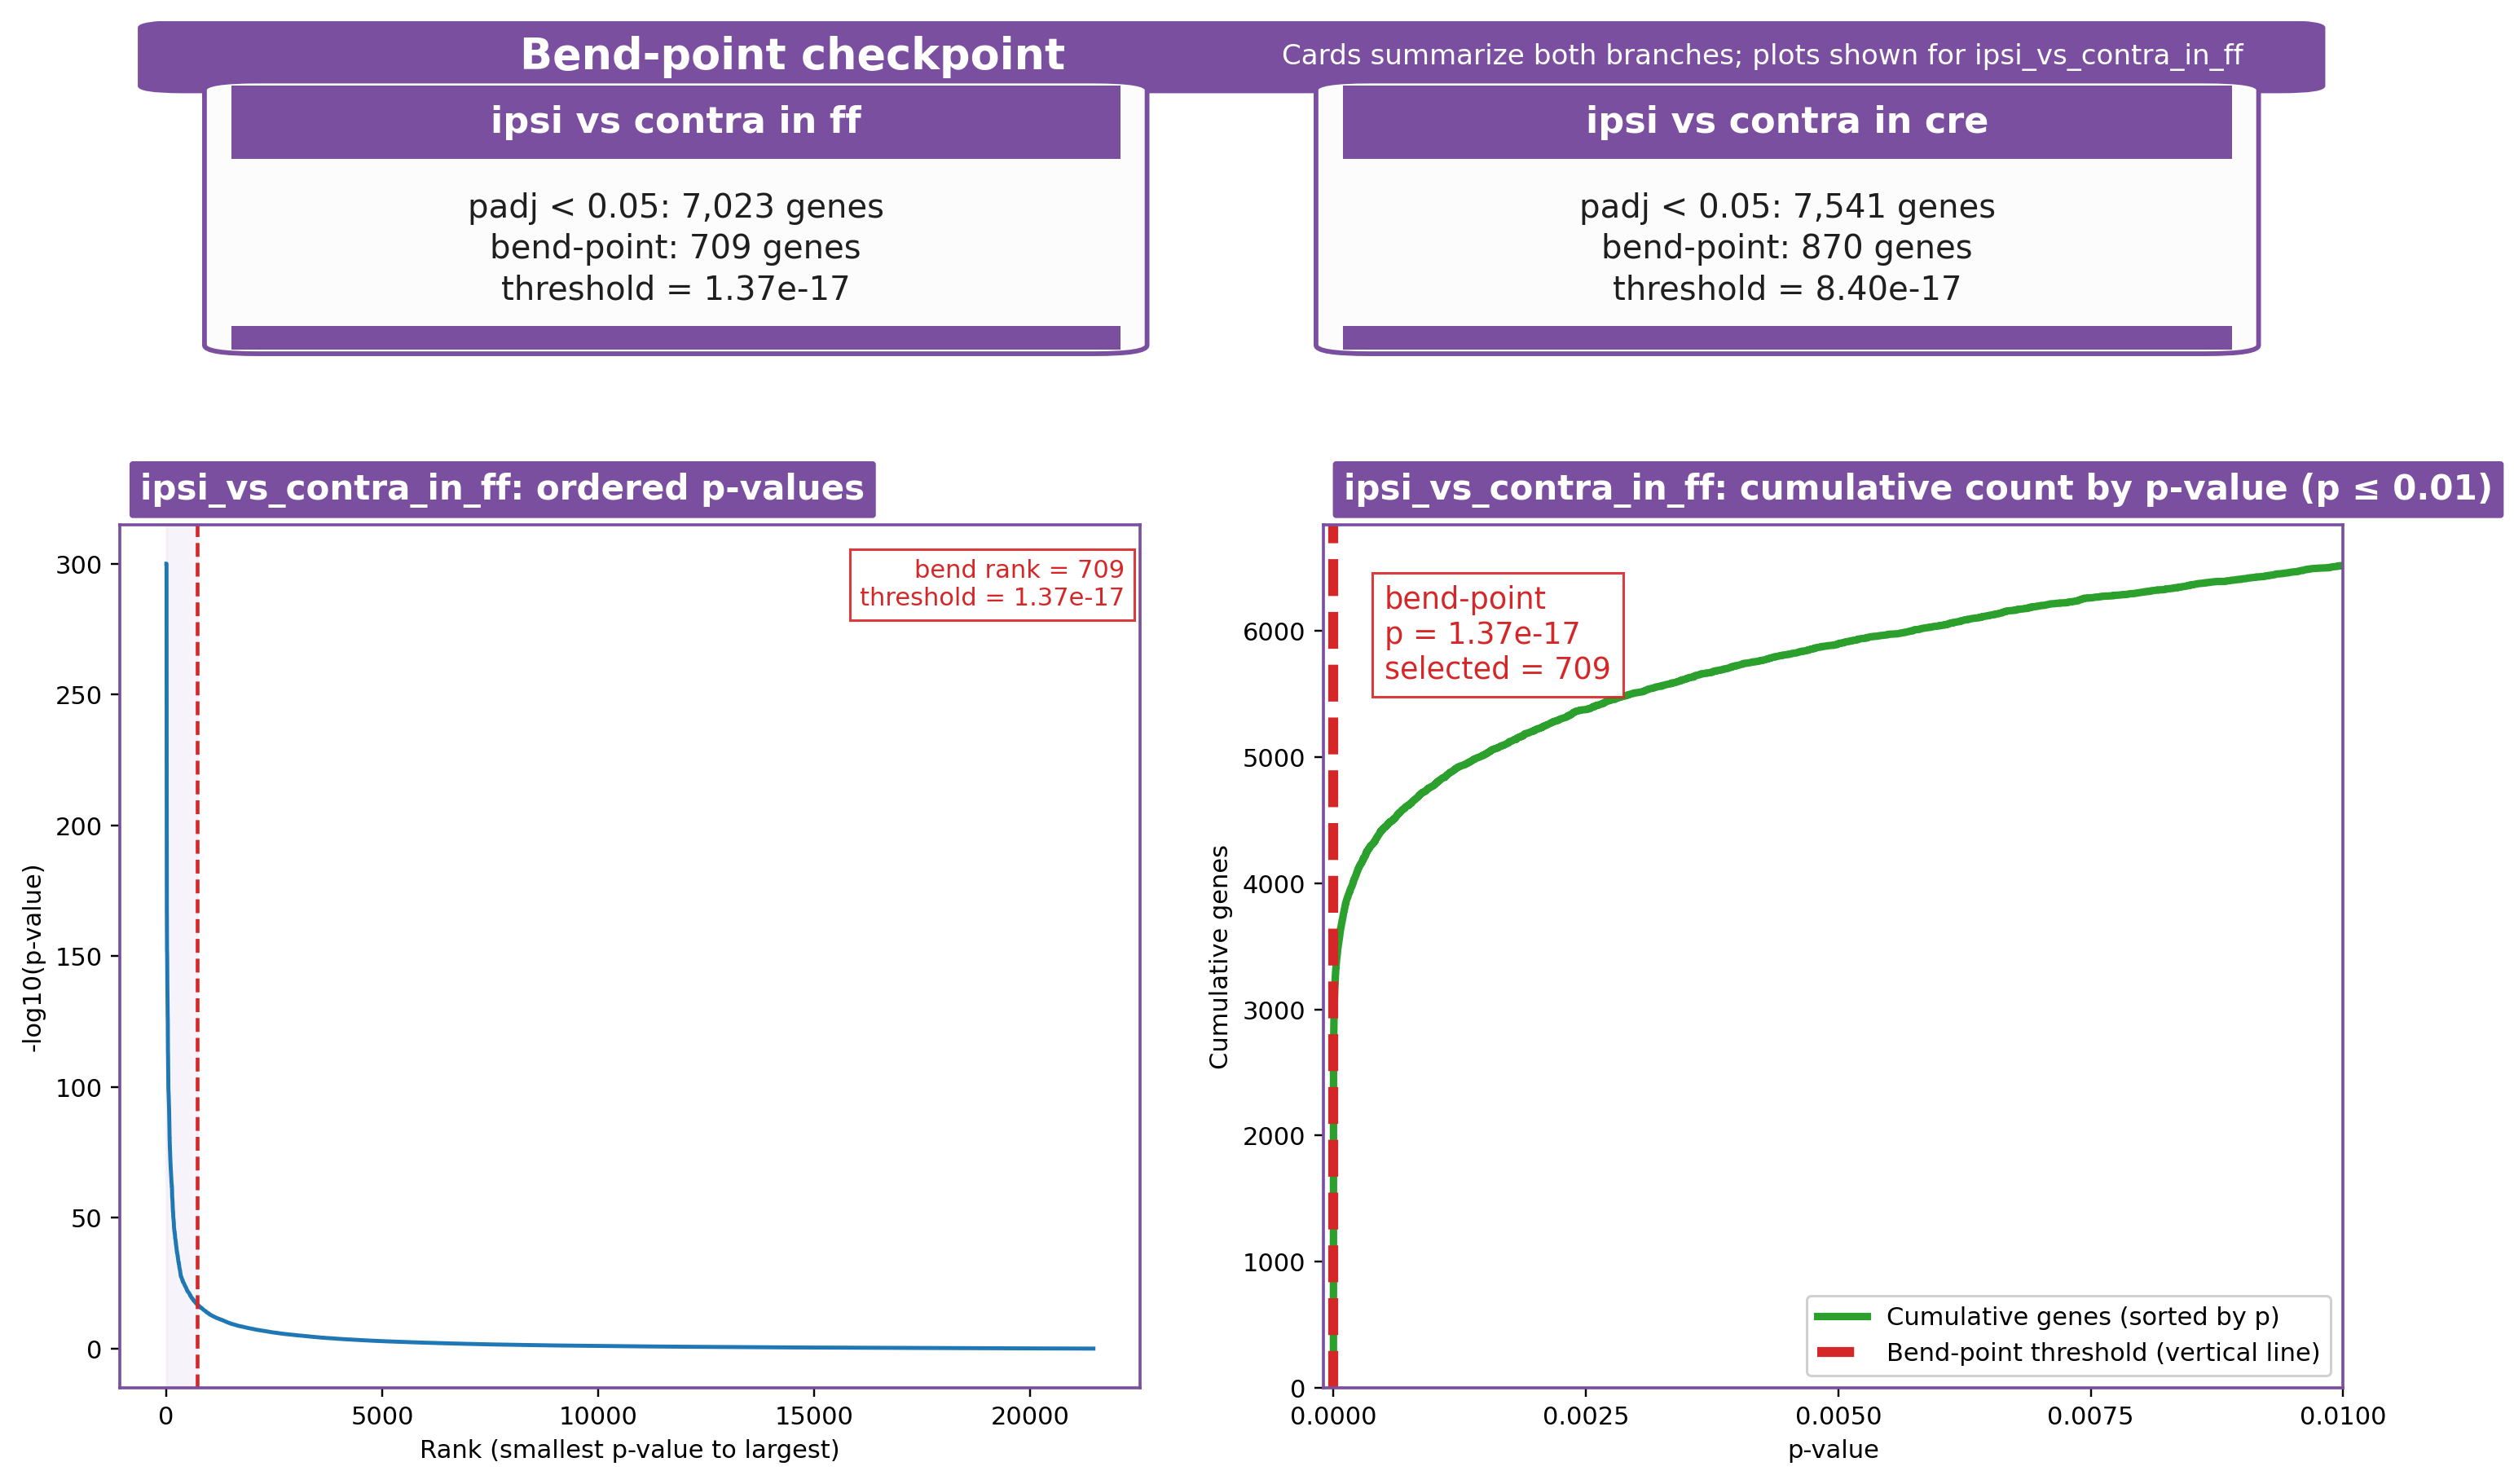
\includegraphics[width=1.04\textwidth]{assets_methods/data_mining_selection_stage.png}
\caption{Retained bend-point checkpoint summary for the two primary side-specific branches (cards). The ordered p-value and cumulative-count plots are shown for the \artifact{ipsi\_vs\_contra\_in\_ff} example, with the right panel zoomed to \textit{p} $\le$ 0.01.}
\label{fig:data_analysis_selection}
\end{figure}

\begin{table}[H]
\centering
\begin{singlespace}
\fontsize{7.1}{8.0}\selectfont
\caption{Data Analysis and Interpretation workflow table.}
\label{tab:data_analysis}
\begin{tabularx}{\textwidth}{Y Y Y Y Y}
\toprule
\rowcolor{tableheader}
\textbf{Substage} & \textbf{Input} & \textbf{Tool} & \textbf{Checkpoint artifact / evidence} & \textbf{Why it mattered} \\
\midrule
\stagecell{stagemine}{Model setup} &
family count matrix + design table &
\artifact{DESeq2} &
normalized counts, VST matrix, and contrast-level result tables; 20 samples retained and 78{,}334 $\rightarrow$ 21{,}481 genes after filtering &
defines the inferential base for every contrast and downstream plot \\

\stagecell{stagemine}{Contrast production} &
filtered model outputs &
\artifact{DESeq2}\\
contrast manifest &
five saved contrast branches; two primary side-specific and three supporting genotype / interaction branches &
keeps the main and supporting stories explicit before list narrowing \\

\stagecell{stagemine}{Bend-point selection} &
ordered adjusted-\textit{p} tables &
local bend-point scripts &
analysis-summary and per-contrast bend-point summary tables; primary side-specific follow-up sets of 709 genes in \artifact{ff} and 870 genes in \artifact{cre} &
turns very large DE lists into smaller reproducible follow-up sets \\

\stagecell{stagemine}{Enrichment layer} &
bend-point-selected gene sets &
\artifact{g:Profiler} &
g:Profiler source-summary and enrichment tables; the main \artifact{ff} branch retained 359 GO:BP, 18 KEGG, and 3 Reactome terms &
captures the terminal functional-summary products without replacing the gene-level story \\
\bottomrule
\end{tabularx}
\end{singlespace}
\end{table}

\begin{table}[H]
\centering
\begin{singlespace}
\fontsize{7.2}{8.0}\selectfont
\caption{Primary side-specific follow-up summary carried out during the Data Analysis stage.}
\label{tab:data_analysis_primary}
\begin{tabularx}{\textwidth}{Y Y Y Y Y Y Y}
\toprule
\rowcolor{tableheader}
\textbf{Branch} & \textbf{\artifact{padj < 0.05} genes} & \textbf{Bend-point genes} & \textbf{Threshold} & \textbf{GO:BP} & \textbf{KEGG} & \textbf{REAC} \\
\midrule
\stagecell{stagemine}{ff side branch} &
\metriccell{stagemine}{7{,}023} &
\metriccell{stagemine}{709} &
\artifact{1.37e-17} &
359 &
18 &
3 \\

\stagecell{stagemine}{cre side branch} &
\metriccell{stagemine}{7{,}541} &
\metriccell{stagemine}{870} &
\artifact{8.40e-17} &
425 &
21 &
7 \\
\bottomrule
\end{tabularx}
\end{singlespace}
\end{table}

\end{document}
